\documentclass{article}

\usepackage{fancyhdr}
\usepackage{extramarks}
\usepackage{amsmath}
\usepackage{amsthm}
\usepackage{amsfonts}
\usepackage{tikz}
\usepackage[plain]{algorithm}
\usepackage{algpseudocode}
\usepackage{graphicx}
\usepackage{csquotes}
\usepackage{caption}
\usepackage{subcaption}
\usepackage{hyperref}
\hypersetup{
    colorlinks=true,
    linkcolor=blue,
    filecolor=blue,
    urlcolor=blue
}

\usetikzlibrary{automata,positioning}

%
% Basic Document Settings
%

\topmargin=-0.45in
\evensidemargin=0in
\oddsidemargin=0in
\textwidth=6.5in
\textheight=9.0in
\headsep=0.25in

\linespread{1.1}

\pagestyle{fancy}
\lhead{\hmwkAuthorName}
\chead{\hmwkClass\ (\hmwkClassInstructor): \hmwkTitle}
\rhead{\firstxmark}
\lfoot{\lastxmark}
\cfoot{\thepage}

\renewcommand\headrulewidth{0.4pt}
\renewcommand\footrulewidth{0.4pt}

\setlength\parindent{0pt}

%
% Create Problem Sections
%

\newcommand{\enterProblemHeader}[1]{
    \nobreak\extramarks{}{Problem \arabic{#1} continued on next page\ldots}\nobreak{}
    \nobreak\extramarks{Problem \arabic{#1} (continued)}{Problem \arabic{#1} continued on next page\ldots}\nobreak{}
}

\newcommand{\exitProblemHeader}[1]{
    \nobreak\extramarks{Problem \arabic{#1} (continued)}{Problem \arabic{#1} continued on next page\ldots}\nobreak{}
    \stepcounter{#1}
    \nobreak\extramarks{Problem \arabic{#1}}{}\nobreak{}
}

\setcounter{secnumdepth}{0}
\newcounter{partCounter}
\newcounter{homeworkProblemCounter}
\setcounter{homeworkProblemCounter}{1}
\nobreak\extramarks{Problem \arabic{homeworkProblemCounter}}{}\nobreak{}

%
% Homework Problem Environment
%
% This environment takes an optional argument. When given, it will adjust the
% problem counter. This is useful for when the problems given for your
% assignment aren't sequential. See the last 3 problems of this template for an
% example.
%
\newenvironment{homeworkProblem}[1][-1]{
    \ifnum#1>0
        \setcounter{homeworkProblemCounter}{#1}
    \fi
    \section{Problem \arabic{homeworkProblemCounter}}
    \setcounter{partCounter}{1}
    \enterProblemHeader{homeworkProblemCounter}
}{
    \exitProblemHeader{homeworkProblemCounter}
}

%
% Homework Details
%   - Title
%   - Due date
%   - Class
%   - Section/Time
%   - Instructor
%   - Author
%

\newcommand{\hmwkTitle}{Assignment\ \#3}
\newcommand{\hmwkDueDate}{October 20, 2020}
\newcommand{\hmwkClass}{SCI 238}
\newcommand{\hmwkClassInstructor}{Dr. Michael Fich}
\newcommand{\hmwkAuthorName}{\textbf{Zach Bortoff}}

%
% Title Page
%

\title{
    \vspace{2in}
    \textmd{\textbf{\hmwkClass:\ \hmwkTitle}}\\
    \normalsize\vspace{0.1in}\small{Due\ on\ \hmwkDueDate\ at 11:59pm}\\
    \vspace{0.1in}\large{\textit{\hmwkClassInstructor}}
    \vspace{3in}
}

\author{\hmwkAuthorName}
\date{}

\renewcommand{\part}[1]{\textbf{\large Part \Alph{partCounter}}\stepcounter{partCounter}\\}

%
% Various Helper Commands
%

% Useful for algorithms
\newcommand{\alg}[1]{\textsc{\bfseries \footnotesize #1}}

% For derivatives
\newcommand{\deriv}[1]{\frac{\mathrm{d}}{\mathrm{d}x} (#1)}

% For partial derivatives
\newcommand{\pderiv}[2]{\frac{\partial}{\partial #1} (#2)}

% Integral dx
\newcommand{\dx}{\mathrm{d}x}

% Alias for the Solution section header
\newcommand{\solution}{\textbf{\large Solution}}

% Probability commands: Expectation, Variance, Covariance, Bias
\newcommand{\E}{\mathrm{E}}
\newcommand{\Var}{\mathrm{Var}}
\newcommand{\Cov}{\mathrm{Cov}}
\newcommand{\Bias}{\mathrm{Bias}}

\begin{document}

\maketitle

\pagebreak

\begin{homeworkProblem}
	The molecules that are trapped in a planet's atmosphere depend on their mass, the planet's mass, the planet's radius, and the planet's temperature. The equation
showing the temperature limit (the planet must be cooler than this to retain the
gas for 100 million years) was given in class. (a) On a log-log plot draw the lines
showing the temperature limits for helium, methane, and carbon dioxide as a
function of M/R (where M is the mass in Earth masses, R is the radius in Earth
Radii). [Plot log(base 10) Temperature on the y axis and log(base 10) M/R on
the x axis. A suggested x-axis range is from M/R of 0.1 to 30. You can label the
axes either in proper log-spaced ticks or in the values that comes from taking the
logs (e.g. -1 to 1.5 for the x-axis).] Show your calculations for one of the
molecules. (b) On this plot add points for the surface/atmospheric temperature of
all of the major planets. (You will need to look these up somewhere. You will
find that this can be a bit confusing! For example some internet sites confuse
average temperature with lowest temperature.) Your final plot will have three
lines (for the molecules) and eight points (one for each planet). (c) Briefly
discuss the retention of atmospheric gases for each planet. Which are far from a
one of the lines? Which are far from a line. What does this mean? (Marks: 6)\\

    \textbf{Solution}

	The orbital data for the planets was obtained from the textbook. The atmospheric temperature data was obtained      \href{(https://solarsystem.nasa.gov/resources/681/solar-system-temperatures/)}{here} (it's a NASA site). All plots and computations were made using Julia. \\
	
    
    (a) To solve this problem, one must first determine the atomic mass units for helium, methane, and carbon, then put those into the below equation: \\
    
    \[
		\begin{split}
			T < 75K \times \frac{m(amu) M / M_{Earth}}{R / R_{Earth}}
		\end{split}
	\]
	
	where,
	
	\[
		\begin{split}
			m_{He} = 2\\
			m_{CH_4} = 16\\
			m_{CO_2} = 44
		\end{split}
	\]
	
	Letting \(x = M/M_{Earth} / R/R_{Earth}\) yields the following linear equation of the limiting temperature with respect to relative Earth Mass-Radius ratio.
	
	\[
		\begin{split}
			T < 75mx
		\end{split}
	\]
	
	Taking the \(log_{10}\) yields:
	
	\[
		\begin{split}
			log_{10}(T) < log_{10}(75m) + log_{10}(x)
		\end{split}
	\]
	
	The \(log_{10}(75m)\) term is constant for each gas, and the \(log_{10}(x)\) term is the same across all the constants. Therefore, we expect each gas to have the same linear slope with an offset corresponding to \(log_{10}(m)\).
	
	Example Computation: Carbon Dioxide at \(M/R\) of 1.0 corresponding to Earth mass and Earth radius.
	
	\[
		\begin{split}
			log_{10}(T) < log_{10}(75 (44)) + log_{10}(1.0) \approx 3.519 + 0.0 \approx 3.519
		\end{split}
	\]\\
	
    (b)
    \begin{figure}[!h]
       	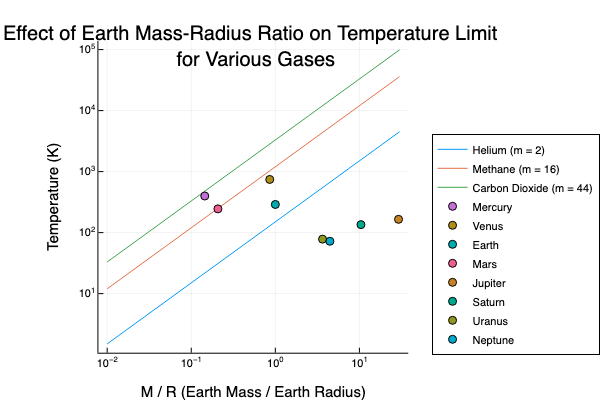
\includegraphics[width=0.9\textwidth]{Q1_LogLogPlot.png}
        	\centering
    		\caption{A Log-Log Plot of Earth mass-Rrdius ratio vs. temperature limit corresponding to helium, methane, and carbon dioxide, supplemented by the points representing each major planet's mass-radius ratio and average temperature. Note that for Mercury, the average temperature was obtained by taking the average between the day-side average and the night-side average. }
    		\label{fig:Plot}
    	\end{figure}
    	
    	(c) To determine whether a given gas will be retained by some planet, one must find all the planets below the given gas line. Correspondingly, all the gas lines above a given planet will be retained by the planet. For example, the gas lines above Earth are methane and carbon dioxide, indicating that the only two gases of the three that can be retained by Earth are \(CO_2\) and \(CH_4\). Similarly, every gas giant lies below every gas, indicating that every gas depicted can be retained by the gas giants. Intuitively, this makes sense, because the gas giants are massive, and have large gravitational fields, which prevent even the smallest of molecules (i.e. \(He\)) from escaping. On the other hand, a small planet like Mercury struggles to retain the heaviest of the three gases, \(CO_2\) and cannot retain either \(CH_4\) or \(He\).
    
    

\end{homeworkProblem}

\pagebreak


\begin{homeworkProblem}
 	Find the properties of a “Least-Energy Orbit” for a spacecraft moving from the
Earth’s orbit to Mars’ orbit. Show your calculations. The spacecraft’s orbit has
its perihelion at the Earth’s orbit and aphelion at Mars’ orbit (assume that both
the Earth’s and Mars’ orbits are perfect circles! Ignore the Earth and Mars
themselves, e.g. any thrust or velocity needed to get away from the Earth’s
gravity.).
(a) Show a sketch of the three orbits (the Earth's, the Mars', and the spacecraft's
orbits)
(b) How long does it take for an unpowered spacecraft to move from Earth's orbit
to Mars' orbit? Give your answer in months.
(c) How fast does the spacecraft need to be moving at the beginning of its trip
(i.e. when it is at the Earth's orbit, but again ignore the Earth itself)?
where M is the mass of the Sun, r is the distance from the Sun (which varies
continuously except in the special case of a circular orbit), and a is the semimajor axis of the orbit. Give your answer in meters/second. (Marks: 4)\\
 	
 	\textbf{Solution}
 	
 	(a)
 	
 	\begin{figure}[!h]
       	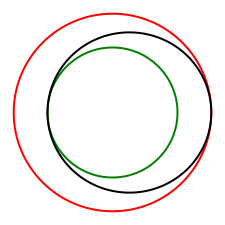
\includegraphics[width=0.25\textwidth]{Q2_PartA_OrbitsDrawing.png}
        	\centering
    		\caption{Drawing of orbits assuming that Mars' and Earth's orbits are circular. Earth's orbit is green, Mars' orbit is red, and the spacecraft orbit is black. }
    		\label{fig:Plot}
    	\end{figure}
 	
 	(b) This problem can be solved by determining the period of the spacecraft's orbit assuming that nothing but the Sun affects the craft's orbit.
 	
 	\[
		\begin{split}
			P^2 = \frac{4\pi}{G(m_1+m_2} a^3\\
			P = 2\pi \sqrt{\frac{a^3}{G M_{Sun}}}
		\end{split}
	\]
	
	We can assume that the spacecraft's mass with respect to the Sun is negligible. The semi-major axis of the spacecraft, \(a\), is given by:
	\[
		\begin{split}
			2a = R_e + R_m\\
			a = \frac{1}{2}(R_e+R_m)
		\end{split}
	\]
	
	where \(R_e\) is the orbital radius of the Earth, and \(R_m\) is the orbital radius of Mars. Now, but looking up the mass of the Sun in the textbook and the orbital radii of the Earth and Mars, we can determine the period and from that the time it takes to get from the perihelion to the aphelion.

	\[
		\begin{split}
			P = 4.46\times10^7 \hspace{3pt}[s]\\
			P/2 = 8.49 \hspace{3pt}[months]
		\end{split}
	\]

\pagebreak
	(c) This problem can be solved by simply applying the following equation, rearranging it for velocity, and then plugging in the values:
	
	\[
		\begin{split}
			v^2 = G(m_1+m_2)( \frac{2}{r} - \frac{1}{a}) \approx G(M_{Sun})(\frac{2}{r_{sun}}-\frac{1}{a})\\
			v \approx \pm \sqrt{G(M_{Sun})(\frac{2}{R_e}-\frac{2}{R_e+R_m})} \approx \pm 32,719\hspace{3pt}[m/s] \\
		\end{split}
	\]
	
	N.B. the plus or minus indicates that the direction of orbit could be changed. 
	
\end{homeworkProblem}

\pagebreak

\end{document}
